\documentclass{article}
\usepackage{polski}
\usepackage{babel}
\usepackage{graphicx}
\usepackage[margin=1in]{geometry}
\usepackage[utf8]{inputenc}
\usepackage{amsmath}
\usepackage{polski}
\usepackage{babel}
\usepackage{hyperref}
\usepackage{graphicx}
\renewcommand{\figurename}{Wykres}
\title{\vspace{4cm} \textbf{Projekt z \\ Projektowania Efektywnych Algorytmów}}
\author{Jakub Grelowski - 262754 \\
        grupa K00-58e \\
        środa - 11:15}
\date{13 grudnia 2022}



\begin{document}

\maketitle

\begin{center}

\large prowadzący: dr inż. Jarosław Mierzwa 

\vspace{1cm}

\Large \textbf{\textit{Zadanie projektowe nr 2 \\ \vspace{1cm} Rozwiązanie problemu komiwojażera za pomocą algorytmu przeszukiwania z ograniczeniami}}     
\end{center}

\vspace{1cm}

\newpage

\tableofcontents

\newpage

\section{Wstęp}
\subsection{Cel projektu}
Celem projektu było napisanie programu umożliwiającego zbadanie analize efektywności algorytmów przybliżonych rozwiązujących asymetryczny problem komiwojażera. 

\subsection{Sposób przechowywania grafów}
\begin{itemize}
    \item Macierz incydencji
\end{itemize}
\subsection{Testowany algorytm}
\begin{itemize}
    \item Przeszukiwanie z ograniczeniami (ang. Tabu search)
\end{itemize}
\subsection{Definicje sąsiedztwa}
\begin{itemize}
    \item Zamiana (ang. Swap)
    \item Wstawianie (ang. Insert)
    \item Odwracanie (ang. Inverse)
\end{itemize}

\subsection{Implementacja}
Do wykonania projektu wykorzystany został język C\# oraz środowisko programistyczne .NET Framework w wersji 4.8.


\section{Reprezentacja grafu w komputerze}
Istnieje kilka różnych sposobów reprezentacji grafu w pamięci komputera. W ramach projektu wykorzystana została macierz incydencji
\subsection{Macierz incydencji}
Macierz incydencji jest macierzą kwadratową o boku $V$, w której wartość $i$–tego wiersza i $j$–tej kolumny jest równa wadze krawędzi $A_{ij}$. Jeśli między dwoma wierzchołkami nie występuje krawędź, wartość na indeksach reprezentujących ją przyjmuje umownie $\infty$, która w programie jest reprezentowana przez 0 bądź -1.




\section{Problem komiwojażera}
Problem komiwojażera to problem obliczeniowy polegający na znalezieniu w grafie cyklu Hamiltona o najmniejszej wadze. Cykl Hamiltona to taki cykl, w którym każdy wierzchołek pojawia się dokładnie raz. 

\subsection{Asymetryczny problem komiwojażera}
Kiedy przeszukiwany graf jest skierowany - czyli waga ścieżki z punktu $A$ do punktu $B$ jest taka sama jak waga ścieżki z punktu $B$ do punktu $A$
 - mówimy wtedy o symetrycznym problemie komiwojażera. Tematem projektu jest jednak asymetryczny problem komiwojażera, czyli sytuacja przeciwna - waga ścieżki z punktu $A$ do punktu $B$ nie jest równa wadze ścieżki z punktu B do punktu A.



\newpage

\section{Przeszukiwanie z ograniczeniami}
\subsection{Algorytm}
Tabu search jest algorytmem metaheurystycznym przeznaczonym do rozwiązywania problemów optymalizacyjnych. Polega on na przeszukiwaniu przestrzenii za pomocą sekwencji ruchów. By uniknąć zapętlania, ruchy zostają zapisane tymczasowo w \textit{liście tabu}. Jeśli ruch w trakcie sprawdzania znajduje się w liście tabu, nie można z niego skorzystać. 

\subsection{Lista tabu}
Do przechowywania ruchów w liście tabu wykorzystana została kolejka przechowująca wykonane ruchy. Po każdym przeszukianiu sąsiedztwa dodawany został najlepszy znaleziony ruch. Jeśli liczba zakazanych ruchów jest większa niż ilość miast, usuwany zostaje najwcześniej dodany ruch.

\subsection{Dywersyfikacja}
By uniknąć przeszukiwania obszaru dziedziny rozwiązań, w którym znalezione zostało minimum lokalne, dodano licznik, który inkrementuje się wtedy, kiedy obecnie znalezione rozwiązanie nie jest lepsze od poprzedniego. W momencie w którym przekroczy on dziesięciokrotność liczby miast, losowana jest nowa ścieżka, a lista tabu jest czyszczona.



\subsection{Definicje sąsiedztwa}

\subsubsection{Zamiana}
Polega na zamianie pozycji $i$-tego oraz $j$-tego miasta w ścieżce.
\subsubsection{Wstawianie}
Polega na wstawieniu $i$-tego miasta w ścieżce na pozycję $j$.
\subsubsection{Odwracanie}
Polega na odwróceniu kolejnością miast pomiędzy miastem $i$ oraz $j$.

\subsubsection{Implementacja}
By zaimplementować różne definicje sąsiedztwa, całość logiki algorytmu zaimplementowano w abstrakcyjnej klasie \textit{TabuSearch}. Następnie utworzono konkretne implementacji tej klasy, takie jak \textit{TabuSearchSwap}, przesłaniające abstrakcyjną metodę \textit{GetNeighbour}.


\section{Najważniejsze klasy w programie}
\begin{itemize}
    \item \textit{TabuSearch} - abstrakcyjna klasa przechowująca większość logiki.
    \item \textit{TabuSearchSwap} - implementacja \textit{TabuSearch} implementująca zamianę pozycjami.
    \item \textit{TabuSearchInsert} - implementacja \textit{TabuSearch} implementująca wstawianie na pozycję.
    \item \textit{TabuSearchInvert} - implementacja \textit{TabuSearch} implementująca odwracanie kolejności.
    \item \textit{Graph} - klasa przechowująca graf w postaci macierzy sąsiedztw oraz jego rozmiar.
    \item \textit{GraphFactory} - klasa generująca losowy graf bądź ładująca graf z pliku tekstowego.
\end{itemize}

\section{Najlepsze znalezione ścieżki}
\subsection{ftv47.atsp}
\subsubsection{Waga}
2196
\subsubsection{Ścieżka}
0, 38, 45, 16, 14, 36, 46, 23, 7, 32, 8, 11, 10, 6, 31, 5, 30, 29, 4, 24, 3, 28, 42, 43, 41, 2, 27, 33, 9, 1, 25, 37, 17, 18, 20, 19, 44, 22, 26, 47, 40, 21, 39, 15, 35, 34, 13, 12, 0
\subsection{ftv170.atsp}

\subsubsection{Waga}
6443
\subsubsection{Ścieżka}
0, 71, 83, 165, 105, 106, 107, 166, 69, 68, 78, 82, 49, 37, 20, 75, 10, 6, 141, 152, 161, 149, 137, 136, 129, 121, 162, 123, 90, 89, 154, 92, 60, 72, 168, 48, 46, 85, 98, 99, 103, 118, 116, 115, 1, 77, 50, 59, 51, 21, 17, 7, 134, 133, 132,
 140, 144, 148, 25, 22, 19, 76, 9, 151, 23, 12, 11, 26, 27, 28, 30, 31, 33, 157, 35, 38, 39, 84, 70, 167, 61, 62, 57, 58, 54, 55, 43, 53, 52, 45, 44, 40, 156, 155, 41, 42, 56, 64, 63, 66, 153, 88, 65, 18, 16, 15, 24, 74, 73, 111, 130, 164, 113, 1
14, 96, 95, 101, 122, 124, 125, 126, 127, 94, 91, 93, 108, 110, 169, 5, 4, 3, 128, 119, 117, 112, 2, 170, 47, 34, 36, 158, 32, 29, 159, 8, 139, 138, 135, 104, 86, 87, 67, 13, 14, 160, 150, 147, 143, 145, 146, 120, 102, 100, 163, 97, 109, 131, 142
, 81, 80, 79, 0
\subsection{ftv170.atsp}
\subsubsection{Waga}
3461
\subsubsection{Ścieżka}
0, 364, 71, 278, 209, 269, 262, 220, 26, 24, 58, 297, 52, 389, 217, 198, 342, 181, 254, 187, 130, 246, 113, 230, 123, 337, 378, 85, 88, 176, 189, 237, 137, 228, 392, 141, 90, 175, 362, 255, 129, 19, 105, 344, 136, 343, 243, 37, 66, 276, 36
1, 302, 245, 30, 184, 93, 29, 401, 122, 128, 368, 260, 172, 388, 109, 191, 252, 281, 294, 326, 195, 295, 296, 49, 166, 21, 22, 160, 6, 20, 159, 68, 340, 152, 69, 14, 11, 41, 34, 203, 387, 43, 377, 63, 13, 247, 288, 134, 38, 309, 355, 311, 155, 39
0, 328, 32, 18, 157, 158, 100, 178, 394, 397, 352, 347, 238, 182, 27, 95, 167, 402, 204, 321, 89, 201, 94, 96, 360, 257, 61, 264, 381, 382, 316, 395, 358, 112, 251, 350, 273, 232, 46, 351, 299, 332, 33, 325, 391, 48, 127, 53, 186, 319, 223, 205,
231, 341, 91, 399, 185, 177, 369, 199, 35, 304, 346, 86, 75, 153, 222, 83, 371, 375, 376, 165, 55, 126, 110, 54, 249, 256, 274, 370, 84, 104, 313, 241, 57, 65, 39, 333, 259, 102, 291, 298, 51, 125, 279, 280, 171, 292, 366, 320, 324, 233, 261, 92,
 214, 8, 336, 147, 156, 77, 210, 47, 3, 163, 174, 265, 101, 28, 372, 384, 150, 239, 67, 221, 74, 312, 224, 240, 168, 307, 329, 284, 170, 383, 62, 114, 131, 398, 200, 354, 4, 213, 211, 400, 119, 300, 385, 290, 330, 190, 379, 60, 7, 59, 140, 266, 3
03, 80, 242, 277, 374, 143, 151, 216, 349, 197, 250, 193, 393, 23, 310, 45, 285, 17, 183, 111, 162, 353, 79, 338, 192, 207, 258, 267, 1, 139, 215, 305, 31, 275, 226, 78, 179, 327, 107, 282, 25, 64, 154, 148, 76, 367, 225, 56, 5, 97, 317, 121, 235
, 229, 244, 359, 180, 365, 308, 118, 268, 173, 345, 219, 82, 73, 306, 132, 87, 161, 42, 98, 16, 188, 272, 322, 357, 287, 106, 15, 164, 253, 323, 331, 289, 363, 81, 234, 50, 286, 263, 169, 144, 146, 149, 318, 283, 212, 227, 236, 138, 396, 334, 373
, 2, 386, 348, 248, 40, 339, 133, 145, 70, 142, 202, 208, 206, 115, 117, 99, 315, 380, 194, 72, 314, 10, 335, 124, 103, 36, 108, 44, 270, 135, 116, 120, 301, 196, 12, 9, 218, 293, 271, 356, 0

\section{Pomiary błędu względnego}
\subsection{ftv47.atsp}
\begin{figure}[h!]
\centering
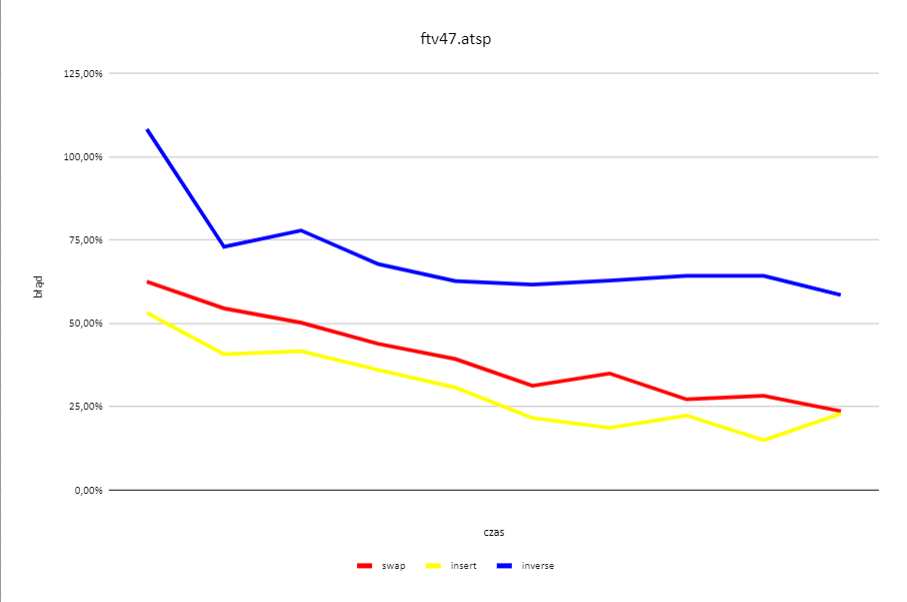
\includegraphics[width=\textwidth]{img/47.png}
\caption{Błąd względny w zależności od czasu - graf ftv47.atsp}
\end{figure}
\newpage
\subsection{ftv170.atsp}
\begin{figure}[h!]
\centering
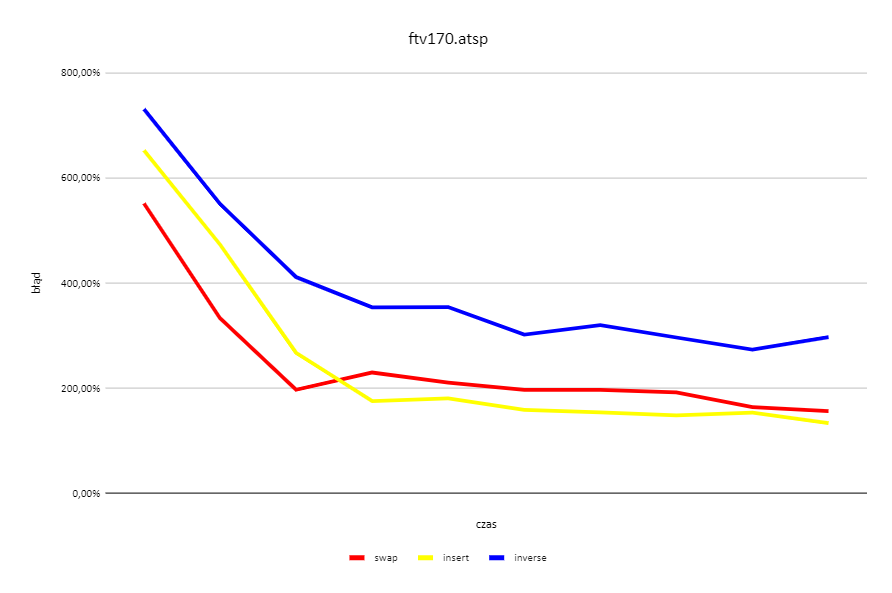
\includegraphics[width=\textwidth]{img/170.png}
\caption{Błąd względny w zależności od czasu - graf ftv170.atsp}
\end{figure}
\newpage
\subsection{rgb403.atsp}
\begin{figure}[h!]
\centering
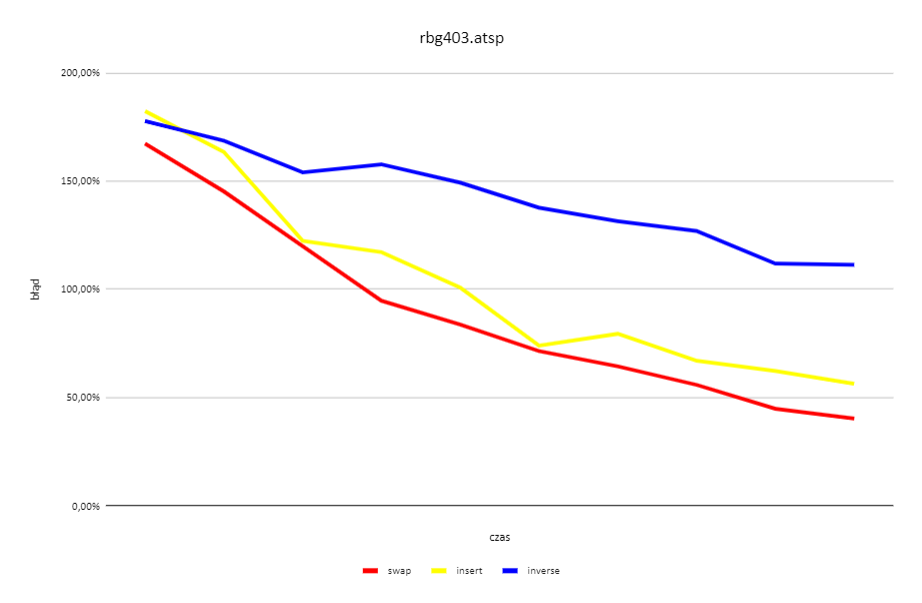
\includegraphics[width=\textwidth]{img/403.png}
\caption{Błąd względny w zależności od czasu - graf rgb403.atsp}
\end{figure}


\section{Wnioski}

Algorytmy zachowywały się zgodnie z oczekiwaniami. 
Z wykresów wynika, że definicja sąsiedztwa $inverse$ wypadała najgorzej - szczególnie dla dłuższego czasu przeszukiwania. \\
Można zauważyć także pewną losowość w zależności błędu i czasu - nie zawsze dłuższy czas przeszukiwania wpływał na lepszy wynik. Wynika to z losowości pierwszej oraz kolejnych ścieżek po dywersyfikacji.

\section{Literatura}

\begin{enumerate}
    \item \url{https://www.ii.uni.wroc.pl/~prz/2011lato/ah/opracowania/szuk_tabu.opr.pdf}
    \item \url{https://en.wikipedia.org/wiki/Tabu_search}
    \item \url{https://cs.pwr.edu.pl/zielinski/lectures/om/localsearch.pdf} 
\end{enumerate}

\end{document}
